\documentclass[tikz,border=5mm]{standalone}
\usepackage{xcolor}

\begin{document}
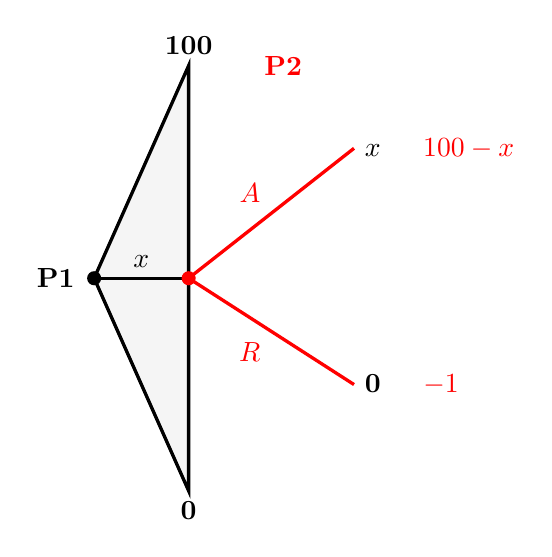
\begin{tikzpicture}[
    scale=1.5,
    font=\bfseries,
    dot/.style={circle, fill=#1, inner sep=1.8pt},
    dot/.default=black,
    line width=1.2pt
]

    % Coordinates
    \coordinate (p1)   at (0, 0);
    \coordinate (top)  at (0.8, 1.8);
    \coordinate (mid)  at (0.8, 0);
    \coordinate (bot)  at (0.8, -1.8);

    \coordinate (leaf_top) at (2.2, 1.1);
    \coordinate (leaf_bot) at (2.2, -0.9);

    % Player 1 continuous action wedge/arc
    \draw[black, fill=gray!8] (p1) -- (top) -- (bot) -- cycle;
    \draw[black] (p1) -- (mid) node[midway, above] {$x$};

    % Continuum labels for Player 1
    \node[above] at (top) {100};
    \node[below] at (bot) {0};

    % Player 2 branches (Red)
    \draw[red] (mid) -- (leaf_top) node[midway, above left] {$A$};
    \draw[red] (mid) -- (leaf_bot) node[midway, below left] {$R$};

    % Nodes & Player labels
    \node[dot=black, label=left:P1] at (p1) {};
    \node[dot=red] at (mid) {};
    \node[red] at (1.6, 1.8) {P2};

    % Payoffs (P1: black, P2: red)
    \node[right] at (leaf_top) {$x$ \quad \textcolor{red}{$100 - x$}};
    \node[right] at (leaf_bot) {0 \quad \textcolor{red}{$-1$}};

\end{tikzpicture}
\end{document}
